% Created by tikzDevice version 0.9 on 2016-01-08 20:52:11
% !TEX encoding = UTF-8 Unicode
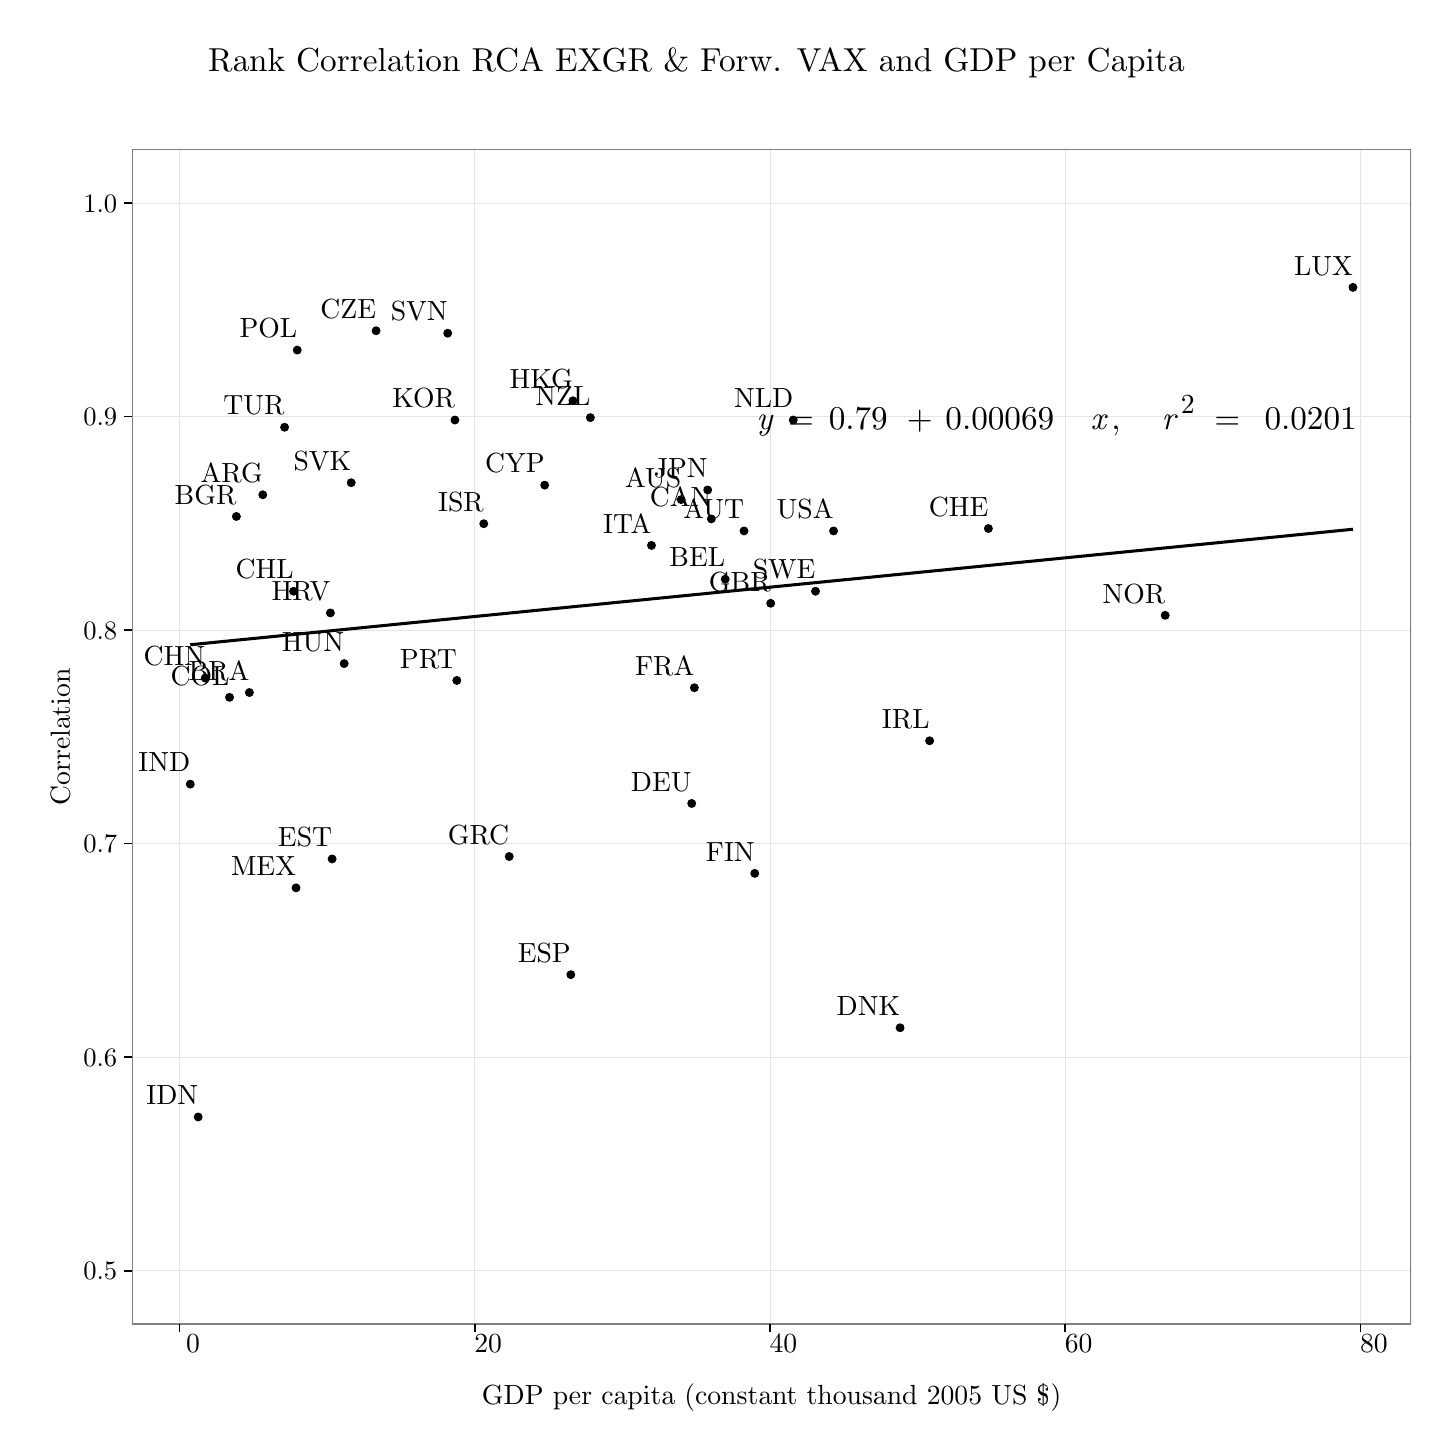
\begin{tikzpicture}[x=1pt,y=1pt]
\definecolor{fillColor}{RGB}{255,255,255}
\path[use as bounding box,fill=fillColor,fill opacity=0.00] (0,0) rectangle (505.89,505.89);
\begin{scope}
\path[clip] (  0.00,  0.00) rectangle (505.89,505.89);
\definecolor{drawColor}{RGB}{255,255,255}
\definecolor{fillColor}{RGB}{255,255,255}

\path[draw=drawColor,line width= 0.6pt,line join=round,line cap=round,fill=fillColor] (  0.00, -0.00) rectangle (505.89,505.89);
\end{scope}
\begin{scope}
\path[clip] ( 37.75, 37.43) rectangle (499.89,461.83);
\definecolor{fillColor}{RGB}{255,255,255}

\path[fill=fillColor] ( 37.75, 37.43) rectangle (499.89,461.83);
\definecolor{drawColor}{gray}{0.90}

\path[draw=drawColor,line width= 0.2pt,line join=round] ( 37.75, 56.72) --
	(499.89, 56.72);

\path[draw=drawColor,line width= 0.2pt,line join=round] ( 37.75,133.88) --
	(499.89,133.88);

\path[draw=drawColor,line width= 0.2pt,line join=round] ( 37.75,211.05) --
	(499.89,211.05);

\path[draw=drawColor,line width= 0.2pt,line join=round] ( 37.75,288.21) --
	(499.89,288.21);

\path[draw=drawColor,line width= 0.2pt,line join=round] ( 37.75,365.38) --
	(499.89,365.38);

\path[draw=drawColor,line width= 0.2pt,line join=round] ( 37.75,442.54) --
	(499.89,442.54);

\path[draw=drawColor,line width= 0.2pt,line join=round] ( 54.87, 37.43) --
	( 54.87,461.83);

\path[draw=drawColor,line width= 0.2pt,line join=round] (161.55, 37.43) --
	(161.55,461.83);

\path[draw=drawColor,line width= 0.2pt,line join=round] (268.23, 37.43) --
	(268.23,461.83);

\path[draw=drawColor,line width= 0.2pt,line join=round] (374.90, 37.43) --
	(374.90,461.83);

\path[draw=drawColor,line width= 0.2pt,line join=round] (481.58, 37.43) --
	(481.58,461.83);
\definecolor{drawColor}{RGB}{0,0,0}
\definecolor{fillColor}{RGB}{0,0,0}

\path[draw=drawColor,line width= 0.4pt,line join=round,line cap=round,fill=fillColor] ( 84.96,337.10) circle (  1.4);

\path[draw=drawColor,line width= 0.4pt,line join=round,line cap=round,fill=fillColor] (236.13,335.36) circle (  1.4);

\path[draw=drawColor,line width= 0.4pt,line join=round,line cap=round,fill=fillColor] (258.85,324.03) circle (  1.4);

\path[draw=drawColor,line width= 0.4pt,line join=round,line cap=round,fill=fillColor] (252.05,306.60) circle (  1.4);

\path[draw=drawColor,line width= 0.4pt,line join=round,line cap=round,fill=fillColor] ( 75.42,329.26) circle (  1.4);

\path[draw=drawColor,line width= 0.4pt,line join=round,line cap=round,fill=fillColor] ( 80.12,265.64) circle (  1.4);

\path[draw=drawColor,line width= 0.4pt,line join=round,line cap=round,fill=fillColor] (247.04,328.38) circle (  1.4);

\path[draw=drawColor,line width= 0.4pt,line join=round,line cap=round,fill=fillColor] (347.15,324.90) circle (  1.4);

\path[draw=drawColor,line width= 0.4pt,line join=round,line cap=round,fill=fillColor] ( 96.09,302.24) circle (  1.4);

\path[draw=drawColor,line width= 0.4pt,line join=round,line cap=round,fill=fillColor] ( 64.15,270.87) circle (  1.4);

\path[draw=drawColor,line width= 0.4pt,line join=round,line cap=round,fill=fillColor] ( 72.93,263.90) circle (  1.4);

\path[draw=drawColor,line width= 0.4pt,line join=round,line cap=round,fill=fillColor] (186.82,340.58) circle (  1.4);

\path[draw=drawColor,line width= 0.4pt,line join=round,line cap=round,fill=fillColor] (125.90,396.36) circle (  1.4);

\path[draw=drawColor,line width= 0.4pt,line join=round,line cap=round,fill=fillColor] (239.94,225.56) circle (  1.4);

\path[draw=drawColor,line width= 0.4pt,line join=round,line cap=round,fill=fillColor] (315.25,144.51) circle (  1.4);

\path[draw=drawColor,line width= 0.4pt,line join=round,line cap=round,fill=fillColor] (196.27,163.69) circle (  1.4);

\path[draw=drawColor,line width= 0.4pt,line join=round,line cap=round,fill=fillColor] (110.01,205.51) circle (  1.4);

\path[draw=drawColor,line width= 0.4pt,line join=round,line cap=round,fill=fillColor] (262.73,200.29) circle (  1.4);

\path[draw=drawColor,line width= 0.4pt,line join=round,line cap=round,fill=fillColor] (240.91,267.38) circle (  1.4);

\path[draw=drawColor,line width= 0.4pt,line join=round,line cap=round,fill=fillColor] (268.48,297.88) circle (  1.4);

\path[draw=drawColor,line width= 0.4pt,line join=round,line cap=round,fill=fillColor] (174.01,206.39) circle (  1.4);

\path[draw=drawColor,line width= 0.4pt,line join=round,line cap=round,fill=fillColor] (197.02,371.08) circle (  1.4);

\path[draw=drawColor,line width= 0.4pt,line join=round,line cap=round,fill=fillColor] (109.40,294.40) circle (  1.4);

\path[draw=drawColor,line width= 0.4pt,line join=round,line cap=round,fill=fillColor] (114.37,276.10) circle (  1.4);

\path[draw=drawColor,line width= 0.4pt,line join=round,line cap=round,fill=fillColor] ( 61.61,112.27) circle (  1.4);

\path[draw=drawColor,line width= 0.4pt,line join=round,line cap=round,fill=fillColor] ( 58.76,232.53) circle (  1.4);

\path[draw=drawColor,line width= 0.4pt,line join=round,line cap=round,fill=fillColor] (325.91,248.21) circle (  1.4);

\path[draw=drawColor,line width= 0.4pt,line join=round,line cap=round,fill=fillColor] (164.81,326.64) circle (  1.4);

\path[draw=drawColor,line width= 0.4pt,line join=round,line cap=round,fill=fillColor] (225.41,318.80) circle (  1.4);

\path[draw=drawColor,line width= 0.4pt,line join=round,line cap=round,fill=fillColor] (245.72,338.84) circle (  1.4);

\path[draw=drawColor,line width= 0.4pt,line join=round,line cap=round,fill=fillColor] (154.39,364.11) circle (  1.4);

\path[draw=drawColor,line width= 0.4pt,line join=round,line cap=round,fill=fillColor] (478.88,412.04) circle (  1.4);

\path[draw=drawColor,line width= 0.4pt,line join=round,line cap=round,fill=fillColor] ( 96.97,195.06) circle (  1.4);

\path[draw=drawColor,line width= 0.4pt,line join=round,line cap=round,fill=fillColor] (276.64,364.11) circle (  1.4);

\path[draw=drawColor,line width= 0.4pt,line join=round,line cap=round,fill=fillColor] (411.04,293.53) circle (  1.4);

\path[draw=drawColor,line width= 0.4pt,line join=round,line cap=round,fill=fillColor] (203.33,364.98) circle (  1.4);

\path[draw=drawColor,line width= 0.4pt,line join=round,line cap=round,fill=fillColor] ( 97.41,389.38) circle (  1.4);

\path[draw=drawColor,line width= 0.4pt,line join=round,line cap=round,fill=fillColor] (155.07,270.00) circle (  1.4);

\path[draw=drawColor,line width= 0.4pt,line join=round,line cap=round,fill=fillColor] (116.91,341.46) circle (  1.4);

\path[draw=drawColor,line width= 0.4pt,line join=round,line cap=round,fill=fillColor] (151.78,395.48) circle (  1.4);

\path[draw=drawColor,line width= 0.4pt,line join=round,line cap=round,fill=fillColor] (284.68,302.24) circle (  1.4);

\path[draw=drawColor,line width= 0.4pt,line join=round,line cap=round,fill=fillColor] ( 92.83,361.50) circle (  1.4);

\path[draw=drawColor,line width= 0.4pt,line join=round,line cap=round,fill=fillColor] (291.20,324.03) circle (  1.4);

\node[text=drawColor,anchor=base east,inner sep=0pt, outer sep=0pt, scale=  1] at ( 84.96,341.54) {ARG};

\node[text=drawColor,anchor=base east,inner sep=0pt, outer sep=0pt, scale=  1] at (236.13,339.80) {AUS};

\node[text=drawColor,anchor=base east,inner sep=0pt, outer sep=0pt, scale=  1] at (258.85,328.47) {AUT};

\node[text=drawColor,anchor=base east,inner sep=0pt, outer sep=0pt, scale=  1] at (252.05,311.04) {BEL};

\node[text=drawColor,anchor=base east,inner sep=0pt, outer sep=0pt, scale=  1] at ( 75.42,333.70) {BGR};

\node[text=drawColor,anchor=base east,inner sep=0pt, outer sep=0pt, scale=  1] at ( 80.12,270.08) {BRA};

\node[text=drawColor,anchor=base east,inner sep=0pt, outer sep=0pt, scale=  1] at (247.04,332.83) {CAN};

\node[text=drawColor,anchor=base east,inner sep=0pt, outer sep=0pt, scale=  1] at (347.15,329.34) {CHE};

\node[text=drawColor,anchor=base east,inner sep=0pt, outer sep=0pt, scale=  1] at ( 96.09,306.68) {CHL};

\node[text=drawColor,anchor=base east,inner sep=0pt, outer sep=0pt, scale=  1] at ( 64.15,275.31) {CHN};

\node[text=drawColor,anchor=base east,inner sep=0pt, outer sep=0pt, scale=  1] at ( 72.93,268.34) {COL};

\node[text=drawColor,anchor=base east,inner sep=0pt, outer sep=0pt, scale=  1] at (186.82,345.03) {CYP};

\node[text=drawColor,anchor=base east,inner sep=0pt, outer sep=0pt, scale=  1] at (125.90,400.80) {CZE};

\node[text=drawColor,anchor=base east,inner sep=0pt, outer sep=0pt, scale=  1] at (239.94,230.00) {DEU};

\node[text=drawColor,anchor=base east,inner sep=0pt, outer sep=0pt, scale=  1] at (315.25,148.96) {DNK};

\node[text=drawColor,anchor=base east,inner sep=0pt, outer sep=0pt, scale=  1] at (196.27,168.13) {ESP};

\node[text=drawColor,anchor=base east,inner sep=0pt, outer sep=0pt, scale=  1] at (110.01,209.96) {EST};

\node[text=drawColor,anchor=base east,inner sep=0pt, outer sep=0pt, scale=  1] at (262.73,204.73) {FIN};

\node[text=drawColor,anchor=base east,inner sep=0pt, outer sep=0pt, scale=  1] at (240.91,271.83) {FRA};

\node[text=drawColor,anchor=base east,inner sep=0pt, outer sep=0pt, scale=  1] at (268.48,302.33) {GBR};

\node[text=drawColor,anchor=base east,inner sep=0pt, outer sep=0pt, scale=  1] at (174.01,210.83) {GRC};

\node[text=drawColor,anchor=base east,inner sep=0pt, outer sep=0pt, scale=  1] at (197.02,375.53) {HKG};

\node[text=drawColor,anchor=base east,inner sep=0pt, outer sep=0pt, scale=  1] at (109.40,298.84) {HRV};

\node[text=drawColor,anchor=base east,inner sep=0pt, outer sep=0pt, scale=  1] at (114.37,280.54) {HUN};

\node[text=drawColor,anchor=base east,inner sep=0pt, outer sep=0pt, scale=  1] at ( 61.61,116.71) {IDN};

\node[text=drawColor,anchor=base east,inner sep=0pt, outer sep=0pt, scale=  1] at ( 58.76,236.97) {IND};

\node[text=drawColor,anchor=base east,inner sep=0pt, outer sep=0pt, scale=  1] at (325.91,252.66) {IRL};

\node[text=drawColor,anchor=base east,inner sep=0pt, outer sep=0pt, scale=  1] at (164.81,331.08) {ISR};

\node[text=drawColor,anchor=base east,inner sep=0pt, outer sep=0pt, scale=  1] at (225.41,323.24) {ITA};

\node[text=drawColor,anchor=base east,inner sep=0pt, outer sep=0pt, scale=  1] at (245.72,343.28) {JPN};

\node[text=drawColor,anchor=base east,inner sep=0pt, outer sep=0pt, scale=  1] at (154.39,368.56) {KOR};

\node[text=drawColor,anchor=base east,inner sep=0pt, outer sep=0pt, scale=  1] at (478.88,416.48) {LUX};

\node[text=drawColor,anchor=base east,inner sep=0pt, outer sep=0pt, scale=  1] at ( 96.97,199.50) {MEX};

\node[text=drawColor,anchor=base east,inner sep=0pt, outer sep=0pt, scale=  1] at (276.64,368.56) {NLD};

\node[text=drawColor,anchor=base east,inner sep=0pt, outer sep=0pt, scale=  1] at (411.04,297.97) {NOR};

\node[text=drawColor,anchor=base east,inner sep=0pt, outer sep=0pt, scale=  1] at (203.33,369.43) {NZL};

\node[text=drawColor,anchor=base east,inner sep=0pt, outer sep=0pt, scale=  1] at ( 97.41,393.83) {POL};

\node[text=drawColor,anchor=base east,inner sep=0pt, outer sep=0pt, scale=  1] at (155.07,274.44) {PRT};

\node[text=drawColor,anchor=base east,inner sep=0pt, outer sep=0pt, scale=  1] at (116.91,345.90) {SVK};

\node[text=drawColor,anchor=base east,inner sep=0pt, outer sep=0pt, scale=  1] at (151.78,399.93) {SVN};

\node[text=drawColor,anchor=base east,inner sep=0pt, outer sep=0pt, scale=  1] at (284.68,306.68) {SWE};

\node[text=drawColor,anchor=base east,inner sep=0pt, outer sep=0pt, scale=  1] at ( 92.83,365.94) {TUR};

\node[text=drawColor,anchor=base east,inner sep=0pt, outer sep=0pt, scale=  1] at (291.20,328.47) {USA};
\definecolor{fillColor}{RGB}{153,153,153}



\path[draw=drawColor,line width= 1.1pt,line join=round] ( 58.76,282.90) --
	( 64.08,283.43) --
	( 69.39,283.96) --
	( 74.71,284.49) --
	( 80.03,285.01) --
	( 85.35,285.54) --
	( 90.67,286.07) --
	( 95.98,286.60) --
	(101.30,287.13) --
	(106.62,287.66) --
	(111.94,288.18) --
	(117.26,288.71) --
	(122.57,289.24) --
	(127.89,289.77) --
	(133.21,290.30) --
	(138.53,290.83) --
	(143.85,291.35) --
	(149.16,291.88) --
	(154.48,292.41) --
	(159.80,292.94) --
	(165.12,293.47) --
	(170.44,293.99) --
	(175.75,294.52) --
	(181.07,295.05) --
	(186.39,295.58) --
	(191.71,296.11) --
	(197.03,296.64) --
	(202.34,297.16) --
	(207.66,297.69) --
	(212.98,298.22) --
	(218.30,298.75) --
	(223.62,299.28) --
	(228.94,299.81) --
	(234.25,300.33) --
	(239.57,300.86) --
	(244.89,301.39) --
	(250.21,301.92) --
	(255.53,302.45) --
	(260.84,302.98) --
	(266.16,303.50) --
	(271.48,304.03) --
	(276.80,304.56) --
	(282.12,305.09) --
	(287.43,305.62) --
	(292.75,306.15) --
	(298.07,306.67) --
	(303.39,307.20) --
	(308.71,307.73) --
	(314.02,308.26) --
	(319.34,308.79) --
	(324.66,309.32) --
	(329.98,309.84) --
	(335.30,310.37) --
	(340.61,310.90) --
	(345.93,311.43) --
	(351.25,311.96) --
	(356.57,312.49) --
	(361.89,313.01) --
	(367.20,313.54) --
	(372.52,314.07) --
	(377.84,314.60) --
	(383.16,315.13) --
	(388.48,315.66) --
	(393.79,316.18) --
	(399.11,316.71) --
	(404.43,317.24) --
	(409.75,317.77) --
	(415.07,318.30) --
	(420.39,318.83) --
	(425.70,319.35) --
	(431.02,319.88) --
	(436.34,320.41) --
	(441.66,320.94) --
	(446.98,321.47) --
	(452.29,321.99) --
	(457.61,322.52) --
	(462.93,323.05) --
	(468.25,323.58) --
	(473.57,324.11) --
	(478.88,324.64);

\node[text=drawColor,anchor=base west,inner sep=0pt, outer sep=0pt, scale=  1.2] at (263.34,360.66) {\itshape y};

\node[text=drawColor,anchor=base west,inner sep=0pt, outer sep=0pt, scale=  1.2] at (274.79,360.66) {=};

\node[text=drawColor,anchor=base west,inner sep=0pt, outer sep=0pt, scale=  1.2] at (289.48,360.66) {0.79};

\node[text=drawColor,anchor=base west,inner sep=0pt, outer sep=0pt, scale=  1.2] at (317.67,360.66) {+};

\node[text=drawColor,anchor=base west,inner sep=0pt, outer sep=0pt, scale=  1.2] at (331.63,360.66) {0.00069};

\node[text=drawColor,anchor=base west,inner sep=0pt, outer sep=0pt, scale=  1.2] at (384.06,360.66) {\itshape x};

\node[text=drawColor,anchor=base west,inner sep=0pt, outer sep=0pt, scale=  1.2] at (391.58,360.66) {,};

\node[text=drawColor,anchor=base west,inner sep=0pt, outer sep=0pt, scale=  1.2] at (395.53,360.66) { };

\node[text=drawColor,anchor=base west,inner sep=0pt, outer sep=0pt, scale=  1.2] at (402.64,360.66) { };

\node[text=drawColor,anchor=base west,inner sep=0pt, outer sep=0pt, scale=  1.2] at (409.76,360.66) {\itshape r};

\node[text=drawColor,anchor=base west,inner sep=0pt, outer sep=0pt, scale=  1.00] at (416.68,366.48) {2};

\node[text=drawColor,anchor=base west,inner sep=0pt, outer sep=0pt, scale=  1.2] at (421.65,360.66) { };

\node[text=drawColor,anchor=base west,inner sep=0pt, outer sep=0pt, scale=  1.2] at (428.77,360.66) {=};

\node[text=drawColor,anchor=base west,inner sep=0pt, outer sep=0pt, scale=  1.2] at (439.83,360.66) { };

\node[text=drawColor,anchor=base west,inner sep=0pt, outer sep=0pt, scale=  1.2] at (446.94,360.66) {0.0201};
\definecolor{drawColor}{gray}{0.50}

\path[draw=drawColor,line width= 0.6pt,line join=round,line cap=round] ( 37.75, 37.43) rectangle (499.89,461.83);
\end{scope}
\begin{scope}
\path[clip] (  0.00,  0.00) rectangle (505.89,505.89);
\definecolor{drawColor}{RGB}{0,0,0}

\node[text=drawColor,anchor=base east,inner sep=0pt, outer sep=0pt, scale=  0.96] at ( 32.35, 53.41) {0.5};

\node[text=drawColor,anchor=base east,inner sep=0pt, outer sep=0pt, scale=  0.96] at ( 32.35,130.58) {0.6};

\node[text=drawColor,anchor=base east,inner sep=0pt, outer sep=0pt, scale=  0.96] at ( 32.35,207.74) {0.7};

\node[text=drawColor,anchor=base east,inner sep=0pt, outer sep=0pt, scale=  0.96] at ( 32.35,284.91) {0.8};

\node[text=drawColor,anchor=base east,inner sep=0pt, outer sep=0pt, scale=  0.96] at ( 32.35,362.07) {0.9};

\node[text=drawColor,anchor=base east,inner sep=0pt, outer sep=0pt, scale=  0.96] at ( 32.35,439.24) {1.0};
\end{scope}
\begin{scope}
\path[clip] (  0.00,  0.00) rectangle (505.89,505.89);
\definecolor{drawColor}{RGB}{0,0,0}

\path[draw=drawColor,line width= 0.6pt,line join=round] ( 34.75, 56.72) --
	( 37.75, 56.72);

\path[draw=drawColor,line width= 0.6pt,line join=round] ( 34.75,133.88) --
	( 37.75,133.88);

\path[draw=drawColor,line width= 0.6pt,line join=round] ( 34.75,211.05) --
	( 37.75,211.05);

\path[draw=drawColor,line width= 0.6pt,line join=round] ( 34.75,288.21) --
	( 37.75,288.21);

\path[draw=drawColor,line width= 0.6pt,line join=round] ( 34.75,365.38) --
	( 37.75,365.38);

\path[draw=drawColor,line width= 0.6pt,line join=round] ( 34.75,442.54) --
	( 37.75,442.54);
\end{scope}
\begin{scope}
\path[clip] (  0.00,  0.00) rectangle (505.89,505.89);
\definecolor{drawColor}{RGB}{0,0,0}

\path[draw=drawColor,line width= 0.6pt,line join=round] ( 54.87, 34.43) --
	( 54.87, 37.43);

\path[draw=drawColor,line width= 0.6pt,line join=round] (161.55, 34.43) --
	(161.55, 37.43);

\path[draw=drawColor,line width= 0.6pt,line join=round] (268.23, 34.43) --
	(268.23, 37.43);

\path[draw=drawColor,line width= 0.6pt,line join=round] (374.90, 34.43) --
	(374.90, 37.43);

\path[draw=drawColor,line width= 0.6pt,line join=round] (481.58, 34.43) --
	(481.58, 37.43);
\end{scope}
\begin{scope}
\path[clip] (  0.00,  0.00) rectangle (505.89,505.89);
\definecolor{drawColor}{RGB}{0,0,0}

\node[text=drawColor,rotate= 0.00,anchor=base,inner sep=0pt, outer sep=0pt, scale=  1.00] at ( 59.74, 27.16) {0};

\node[text=drawColor,rotate= 0.00,anchor=base,inner sep=0pt, outer sep=0pt, scale=  1.00] at (166.42, 27.16) {20};

\node[text=drawColor,rotate= 0.00,anchor=base,inner sep=0pt, outer sep=0pt, scale=  1.00] at (273.10, 27.16) {40};

\node[text=drawColor,rotate= 0.00,anchor=base,inner sep=0pt, outer sep=0pt, scale=  1.00] at (379.77, 27.16) {60};

\node[text=drawColor,rotate= 0.00,anchor=base,inner sep=0pt, outer sep=0pt, scale=  1.00] at (486.45, 27.16) {80};
\end{scope}
\begin{scope}
\path[clip] (  0.00,  0.00) rectangle (505.89,505.89);
\definecolor{drawColor}{RGB}{0,0,0}

\node[text=drawColor,anchor=base,inner sep=0pt, outer sep=0pt, scale=  1.00] at (268.82,  8.40) {GDP per capita (constant thousand 2005 US \$)};
\end{scope}
\begin{scope}
\path[clip] (  0.00,  0.00) rectangle (505.89,505.89);
\definecolor{drawColor}{RGB}{0,0,0}

\node[text=drawColor,rotate= 90.00,anchor=base,inner sep=0pt, outer sep=0pt, scale=  1.00] at ( 15.29,249.63) {Correlation};
\end{scope}
\begin{scope}
\path[clip] (  0.00,  0.00) rectangle (505.89,505.89);
\definecolor{drawColor}{RGB}{0,0,0}

\node[text=drawColor,anchor=base west,inner sep=0pt, outer sep=0pt, scale=  1.2] at ( 65.19,489.97) {Rank Correlation RCA EXGR \& Forw. VAX and GDP per Capita};
\end{scope}
\end{tikzpicture}
